\chapter{Current UCN Facility at TRIUMF\label{chap:UCNattriumf}}

% Based on simulations, a 40~$\mu$A of current produces a background of
% XXX mSev.

The current vertical UCN cryostat at TRIUMF is the same UCN cryostat
developed and tested at KEK-RCNP, In October 2016, the cryostat was
shipped to triumf and in 2017 it was installed at a dedicated
spallation neutron source for further UCN experiments. The main
purpose of such experiments were for better understanding of the
vertical UCN source and the design of the next generation UCN source
for higher statics. The 520~MeV cyclotron at TRIUMF provides up to
40~$\mu$A of proton beam that can be diverted onto a tungsten
spallation target. The vertical UCN source is placed above the target
and is surrounded by graphite blocks serving as neutron reflectors.


The vertical source was modified to fulfill the Canadian safety
requirements at TRIUMF. Those include installing pressure relief
valves on the cryostat and the UCN guides and additional radiation
shielding. The extra shielding requires much longer UCN guides
compared to RCNP. The current location of the vertical source is at
the meson hall experimental area. A map of TRIUMF is shown in
Fig.~\ref{fig:sitemap}.

\begin{figure}[h!]
  \centering
  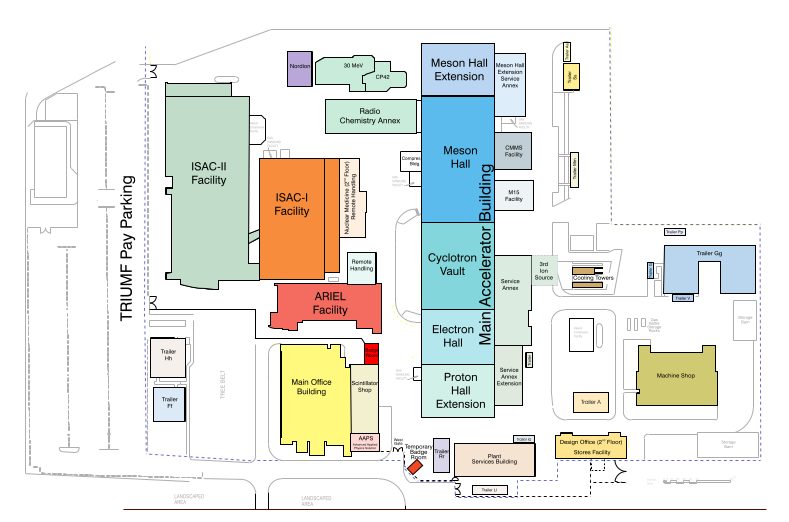
\includegraphics[width=1.0\textwidth]{sitemap.png}
  \caption{A map of TRIUMF. The UCN facility is located at the Meson
    Hall area shown in Blue.}
  \label{fig:sitemap}
\end{figure}

The unique feature of the UCN source at TRIUMF is the combination of
spallation neutrons and superfluid helium for UCN production. The
important elements of the UCN facility at TRIUMF are presented below.
%%%%%%%%%%%%%%%%%%%%%%%%%%%%%

%%%%%%%%%%%%%%%%%%%%%%%%%%%%%
\section{UCN Beam Line~(BL1U)}
TRIUMF produces negatively charged hydrogen ions from an ion
source. These ions are then accelerated in the 520~Mev cyclotron in an
outward spiral trajectory. A thin graphite stripper foil removes the
electrons from the hydrogen ion while protons can pass through. The
proton, because it is a positively charged particle, is deflected in
the outward direction due to the magnetic field and is directed to a
proton beam line. The cyclotron has three independent extraction
probes with various sizes of foils to provide protons to up to three
beam lines~(BL) simultaneously~(see Fig.~\ref{fig:cyclotron}).

\begin{figure}[h!]
  \centering
  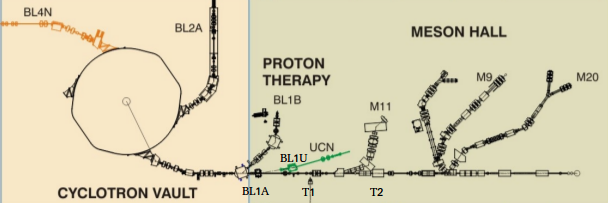
\includegraphics[width=0.8\textwidth]{cyclotron.png}
  \caption{TRIUMF cyclotron and the three beam lines.}
  \label{fig:sitemap}
\end{figure}


The 120~$\mu$A beam (BL1A) enters the Meson Hall, routinely delivers
protons at 480~MeV to two target systems: T1 and T2 for the $\mu$SR
experimental channels. Beam line 1B~(BL1B) separates off BL1 at the
edge of the cyclotron vault and provides international users with the
Proton Irradiation Facility (PIF), which mimics space radiation for
testing computer chips.  The new BL1U provides beam to the UCN
source. BL2A provides 480~MeV proton beams for the targets that
produce exotic ion beams for a host of experiments in ISAC.


The microstructure of BL1A is in pulses with approximately 1~ms
periods of beam followed by a 50-100~$\mu$s periods of no beam.  This
is shown in Fig.~(\ref{fig:bl1u})~\cite{Nick_thesis}.  A kicker magnet
and the septum magnet kick away 1/3 of the beam from BL1A to BL1U and
transport it to a conventional dipole~(bender) magnet~(See
Fig.~\ref{fig:magnets}).

\begin{figure}[h!]
  \centering
  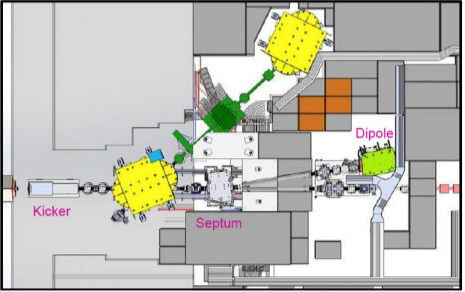
\includegraphics[width=0.9\textwidth]{magnets.png}
  \caption{The kicker, septum and dipole (bender) magnets define the
    front two sections of BL1U.}
  \label{fig:magnets}
\end{figure}
The vertical UCN cryostat is sitting above the tungsten target and is
designed for a maximum of 40~$\mu$A beam on target. As a result, only
one third of the beam can go to the UCN experimental area and the rest
is shared with other users.

\begin{figure}[h!]
  \centering
  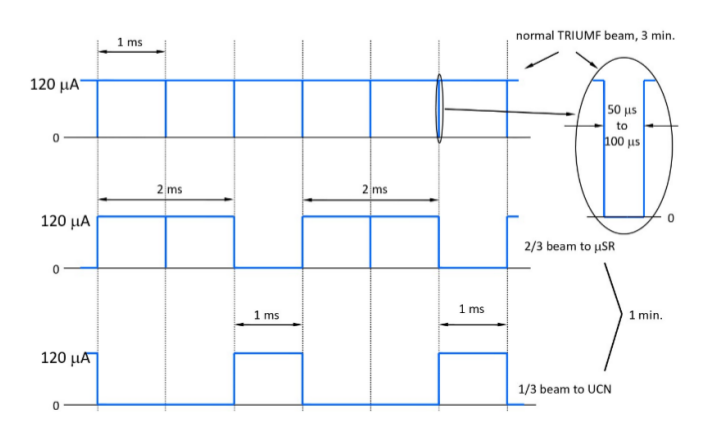
\includegraphics[width=0.9\textwidth]{bl1u.png}
  \caption{UCN beam structure. The top graph shows the 120~$\mu$A BL1A
    in 1~ms period of beam followed by a 50-100~$\mu$s of no
    beam. The middle graph shows the same beam line when the kicker
    magnet is on. The bottom graph shows the 1/3 of the beam that goes
    to the UCN area.}
  \label{fig:bl1u}
\end{figure}

After the bender magnet, the beam then passes through a cored
shielding block and reaches the two quadrupole magnets providing the
final focus of the beam onto a 12~cm thick tungsten spallation target.
The target is located inside a hermetically-sealed target crypt, which
also envelops the beam line exit window that defines the end of BL1U.
Upstream of the beam line window, there is a collimator to reduce the
halo from the proton beam, as well as to help reduce the amount of
neutrons and photons streaming back into the beam line from the target
region~(the collimator also increases the impedance for the passage of
gas arising from any target or window failure, to allow time for the
cyclotron fast valves to close). This last part of the beam line also
contains a variety of beam position and current monitors. The
spallation target and UCN source, located downstream of the beam
line-exit window, are enclosed in a large shielding
pyramid~Fig~\ref{fig:pyramid}.
\begin{figure}[h!]
  \centering
  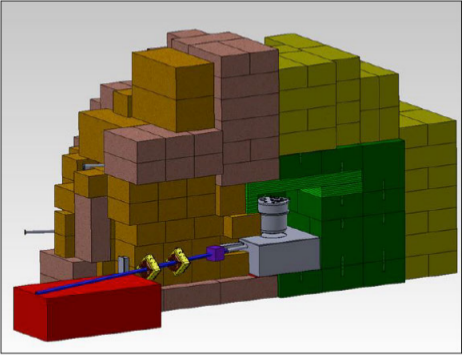
\includegraphics[width=0.8\textwidth]{pyramid.png}
  \caption{Two quadrupole magnets which focus the proton beam onto a
    12~cm thick tungsten spallation target, located inside a
    hermetically-sealed target crypt. Also shown is the UCN shielding
    pyramid, which encases both the spallation target and the UCN
    source, and is designed to meet the dose rate requirements
    specified by the TRIUMF Safety Group.}
  \label{fig:pyramid}
\end{figure}

\section{Tungsten Spallation Target\label{sec:target}}
The spallation target is located at the downstream end of BL1U. The
UCN spallation target comprises a series of rectangular blocks, adding
up to roughly one stopping length~(11~cm) of tungsten, with a
cross-section of $\sim6 \times 8$~cm$^2$~(see
Fig.~\ref{fig:target}). This geometry is very similar to~(and
motivated by) the neutron spallation target design used at KEK (KENS
facility)~\cite{kawai2001fabrication}. The target requires a support
and cooling system, and is designed to allow for remote-handling and
ease of servicing. The target-cooling and remote-handling systems are
designed for an instantaneous proton current of 40~$\mu$A~(10~$\mu$A
time-averaged).
\begin{figure}[h!]
  \centering
  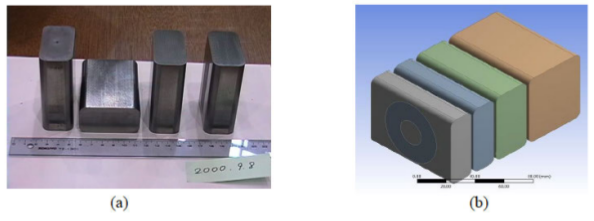
\includegraphics[width=0.8\textwidth]{target.png}
  \caption{(a) Tungsten Target Blocks from the spallation target at
    KEK. The target blocks are plated with tantalum. (b) Present
    design for the tungsten spallation target at the TRIUMF UCN
    facility. The target blocks have a cross-section of
    $5.7 \times 7.8$~cm$^2$ , and thicknesses of 2.0, 2.0, 3.0, and
    5.0~cm, respectively.}
  \label{fig:target}
\end{figure}
The target is being water-cooled. A coating of tantalum prevents
corrosion by the water cooling system. An extraction system allows to
exchange the target when necessary.

%\section{Radiation Sheilding}
% I am not sure if there is anything specific about shielding to
% say. It comes with moderators and when I show the figures of the
% experimental area it will be mentioned.

%%%%%%%%%%%%%%%%%%%%%%%%%%%%%%%%%%%%%%%%%%%%%%%%%%%
%%% JUST TALKING ABOUT THE SETUP
%%%%%%%%%%%%%%%%%%%%%%%%%%%%%%%%%%%%%%%%%%%%%%%%%%%
\section{Vertical UCN Source at TRIUMF\label{sec:vertical_source}}
Neutrons are produced through the spallation process by hitting a
Tungsten target by the proton beam. Spallation is refered
to a nuclear reaction where high energy particles interact with atomic
nucleus. This process creates many high energy neutrons and background
radiation. The target is surrounded by several blocks of lead and
graphite. The fast neutrons are reflected and moderated down and enter
the warm D$_2$O moderator at room temperature~(300~K) and become
thermal neutrons with an energy of 0.025~eV and the speed of 2.2~km/s.
Iced heavy water at 10~K is used as a cold moderator. After passing
through the warm D$_2$O, thermal neutrons enter the the cold moderator
and become cold neutrons. These neutrons have the speed of several
hundreds of meter per second.  UCN are produced when the slow neutrons
enter the isotopically pure superfluid helium at 0.84 to 0.92~K as a
result of phonon transitions inside the superfluid helium as discussed
in section~\ref{sec:ucn_with_heII}.

The schematic of the vertical source is shown in
Fig.~\ref{fig:source}.  The neutron moderators and the helium
circulation system are explained below.


\begin{figure}[h!]
  \centering
  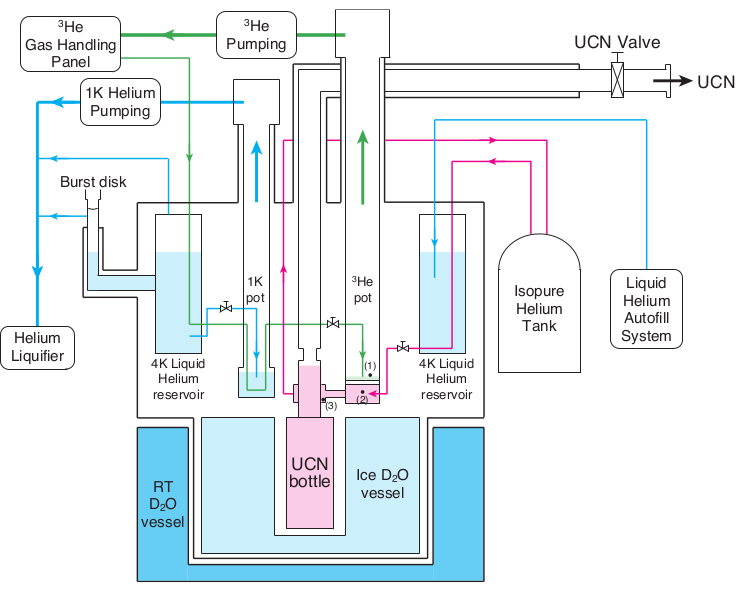
\includegraphics[width=0.9\textwidth]{vertical_source.png}
  \caption{Schematic diagram of the vertial UCN source at
    TRIUMF. Spallation neutrons are moderated in warm D$_2$O vessel
    and become cold neutrons in Iced D$_2$O. The cold neutrons then
    enter the superfluid helium bottle where they become UCN by phonon
    excitations in the superfluid. The isotopically pure superfluid
    helium is cooled down to below 1~K via a $^3$He pot. The $^3$He
    pot is cooled down to 0.7~K via 1~K pot and further pumping. The
    detailed explanation is available in the text. }
  \label{fig:source}
\end{figure}


\subsection{Neutron D$_2$O Moderators}
Deuterium is an isotope of hydrogen which has one proton and one
neutron in the nucleus and it has a lower probability to absorb
neutrons. As a result heavy water is used as a neutron moderator. The
warm D$_2$O moderator to create thermal neutrons from spallation
neutrons is at room temperature. However the cold moderator for the
production of cold neutrons is at much lower
temperature~($\sim$~10~K).

\subsubsection{D$_2$O Solidification}
The Iced D$_2$O vessel has a capacity of 100~L. About 14~L of liquid
D$_2$O is injected to the vessel initially. This is followed by adding 11~L of
D$_2$O to the vessel over 8 times.  After filling up the vessel,
Gifford McMahon refrigerators solidify the heavy water and further
cool it down to 20~K. The process of icing the heavy water takes about
6 days and cooling it down to 20~k takes another 7 days.

%%%%%%%%%%%%%%%%%%%%%%%%%%%%%%%%%%%%%%%%%%%%%%%%%%%
% This is where I left off and where I should start
% again on Monday

\subsection{Helium Circulation and Superfluid Helium Condensation}
The helium circulation and the condensation of the superfluid helium
could be started once the temperature of D$_2$O is as low as 10~K. The
stages towars superfluid helium condensation is presented below. The
full operation and desing detail are available in
Ref.~\cite{matsumiya_thesis}.

\subsubsection{4 Kelvin Reservoir}
The first step of the helium circulation is to fill up the helium
reservoir with the commercially available 4.2~K helium. The full
capacity of the helium reservoir is 50~L. In the 2017 experimental
run, the TUCAN collaboration used a labview program to automatically
fill up the reservoir using a 500~L dewar of 4.2~K helium. This was
refered to as the {\it{stationary dewar}}. This way, it is possible to
set the minimum and maximum levels of the available helium. The helium
levels were measured by two level meters and two flow meteres. The DAQ
system and sensor positions are described in Sec.~\ref{sec:DAQ}.  The
stationary dewar was filled up with 350~L dewars~({\it{transport
    dewar}}) of 4~K helium from the meson hall liquifier. The helium
autofill system is shown in Fig.~\ref{fig:ucnarea}.

\begin{figure}[h!]
  \centering
  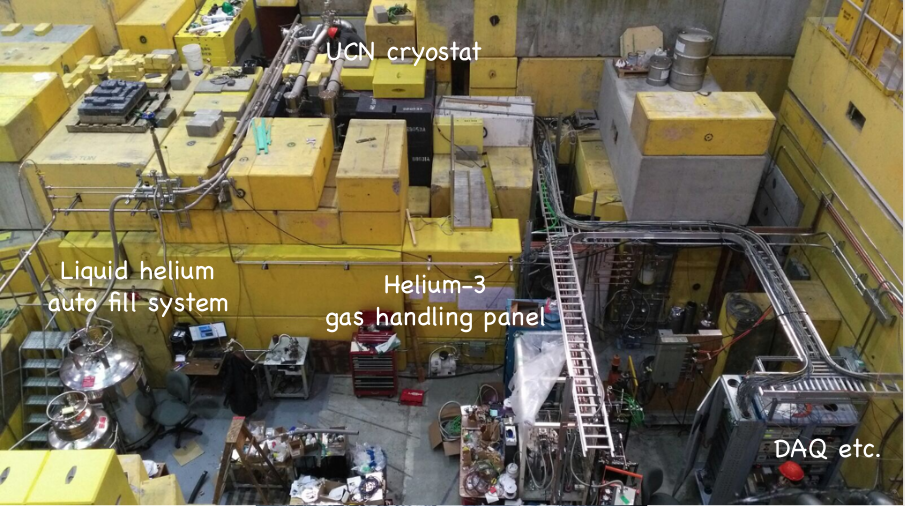
\includegraphics[width=0.9\textwidth]{ucnarea.png}
  \caption{A photograph of the UCN experimental area during the mini
    shutdown in October 2017. The location of some experimental parts
    are shown via labels. The yellow concrete blocks are blocking the
    radiation during beam on target. The UCN vertical cryostat could
    be seen because of the removal of the shield. }
  \label{fig:ucnarea}
\end{figure}

Fig.~\ref{fig:4kfilling} shows the 5 filling cycles of the 4~K
reservoir on April 22 2017 during the first cool down test. The liquid
helium transfer starts once the liquid level in the 4~K reservoir
reaches 20\%. Once the transfer starts, the liquid level starts to
decrease with a sharper slope. The reason for this behaviour is
introducing heat load to the reservoir. It takes some time to cool
down the transfer line from the stationary dewar to the reservoir and
the warm liquid helium causes a boil off in the 4~K reservoir. The
boiled off helium goes through the recovery line to the liquifier. The
liquid helium transfer stops once the 4~K reservoir is filled to about
60\%.

\begin{figure}[h!]
  \centering
  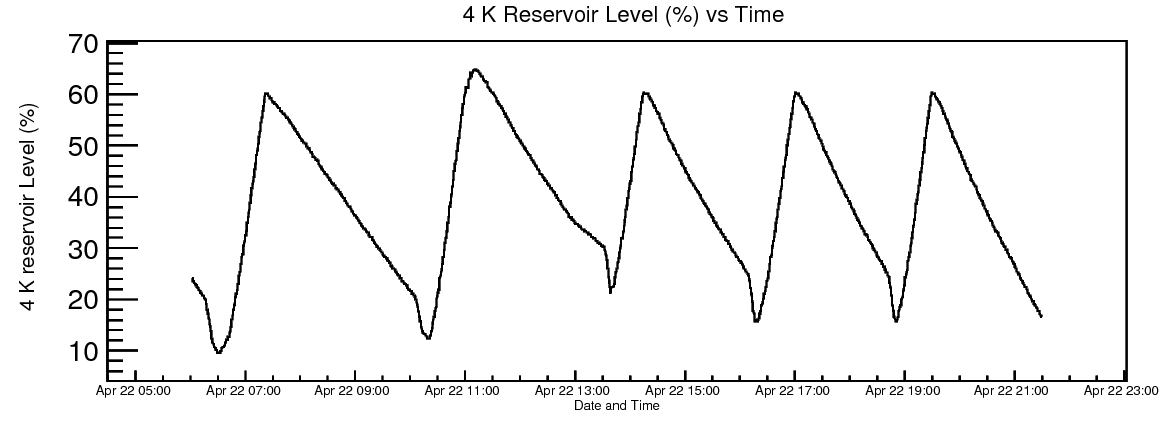
\includegraphics[width=1.0\textwidth]{april_4kfilling.png}
  \caption{The 4~K reservoir filling during the cool down test in April 2017.}
  \label{fig:4kfilling}
\end{figure}
The efficiency of each transfer from the stationary dewar to the 4~K
reservoir was about 40\% to 60\% on average.

\subsubsection{1 Kelvin Pot}
The 4.2~K liquid helium in the helium reservoir is transported to a
pot called {\it{1~K pot}}. The flow rate of the transported liquid
helium is controlled by a needle valve. The 1~K pot is always pumped
by a pumping system to cool the 4.2~K helium down to about 1.4~K. The
level of helium in the 1~K pot is measured by a liquid level
meter. The maximum level of the 1.4 K liquid helium is about 15~cm. At
this level, the volume of the 1.4~K liquid helium is about 1.3~L.


\subsubsection{$^3$He Pot}
Once the 1~K pot is ready the $^3$He circulation starts to condense
into the {\it{$^3$He pot}}. To start, the valve of the $^3$He
reservoir is opened. A vaccum pump compresses the $^3$He gas. The
$^3$He gas is then purified by a room temperature and a cold purifier
and enters the 4~K reservoir to be precooled. The further cooling down
to 1~K and condensation happen via the 1~K pot. The liquid $^3$He is
then transported to $^3$He pot and further cooled down to 0.7~K via
pumping. The evaporated $^3$He is pumped out and goes through an oil
filter and goes back to the beginning point of the circulation.

\subsubsection{Isopure Helium}
After filling the $^3$He pot with 0.7~K liquid $^3$He, the
condensation of isotopically pure~(isopure) superfluid helium
starts. The isopure helium has much less $^3$He than $^4$He~(less than
$10^{-10}$).  Even though the natural abundance of $^3$He is
$1.37 \times 10^{-6}$ in the atmosphere, this value is still large
because of the large neutron absorption cross section of $^3$He. The
existence of $^3$He causes the UCN storage lifetime to decrease~(see
Sec.~\ref{sec:basic_idea}).

The isopure helium is stored in the {\it{isopure helium tank}} shown
in Fig.~\ref{fig:source}. Before entering the cryostat, the
isopure helium goes through a purifier. The purifier is composed of
low temperature charcoals cooled by LN$_2$.  The isopure He is
precooled in the 4~K reservoir and goes into the heat exchange pot
attached to the bottom of the $^3$He cryostat. The bottom of the
$^3$He cryostat and the top of the heat exchange pot is connected via
the copper heat exchanger. The isopure He in the heat exchange pot is
cooled by the 0.7~K liquid $^3$He via the Cu heat exchanger and
becomes He-II. The condensed He-II fills the He-II bottle with a
volume of 8.5~L and gets cooled down to $\sim$~0.83~K.




\section{Data Acquisition System\label{sec:DAQ}}
The TUCAN UCN DAQ system accumulates data from different devices and
integrates them into a MIDAS file.

For the 2017 data acquisition, almost all the sensors such as
temperature sensors, flow meteres, pressure gaugas and {\it{etc.}}
were connected to a Programmable Logic Controller~(PLC).  The PLC
receives information from the connected sensors or input devices,
processes the data, and triggers outputs based on pre-programmed
parameters.  Depending on the inputs and outputs, a PLC can monitor
and record data, automatically start and stop processes, generate
alarms based on the applied limits, and more. A picture of the PLC is
shown in Fig.~\ref{fig:PLC}.

\begin{figure}[h!]
  \centering
  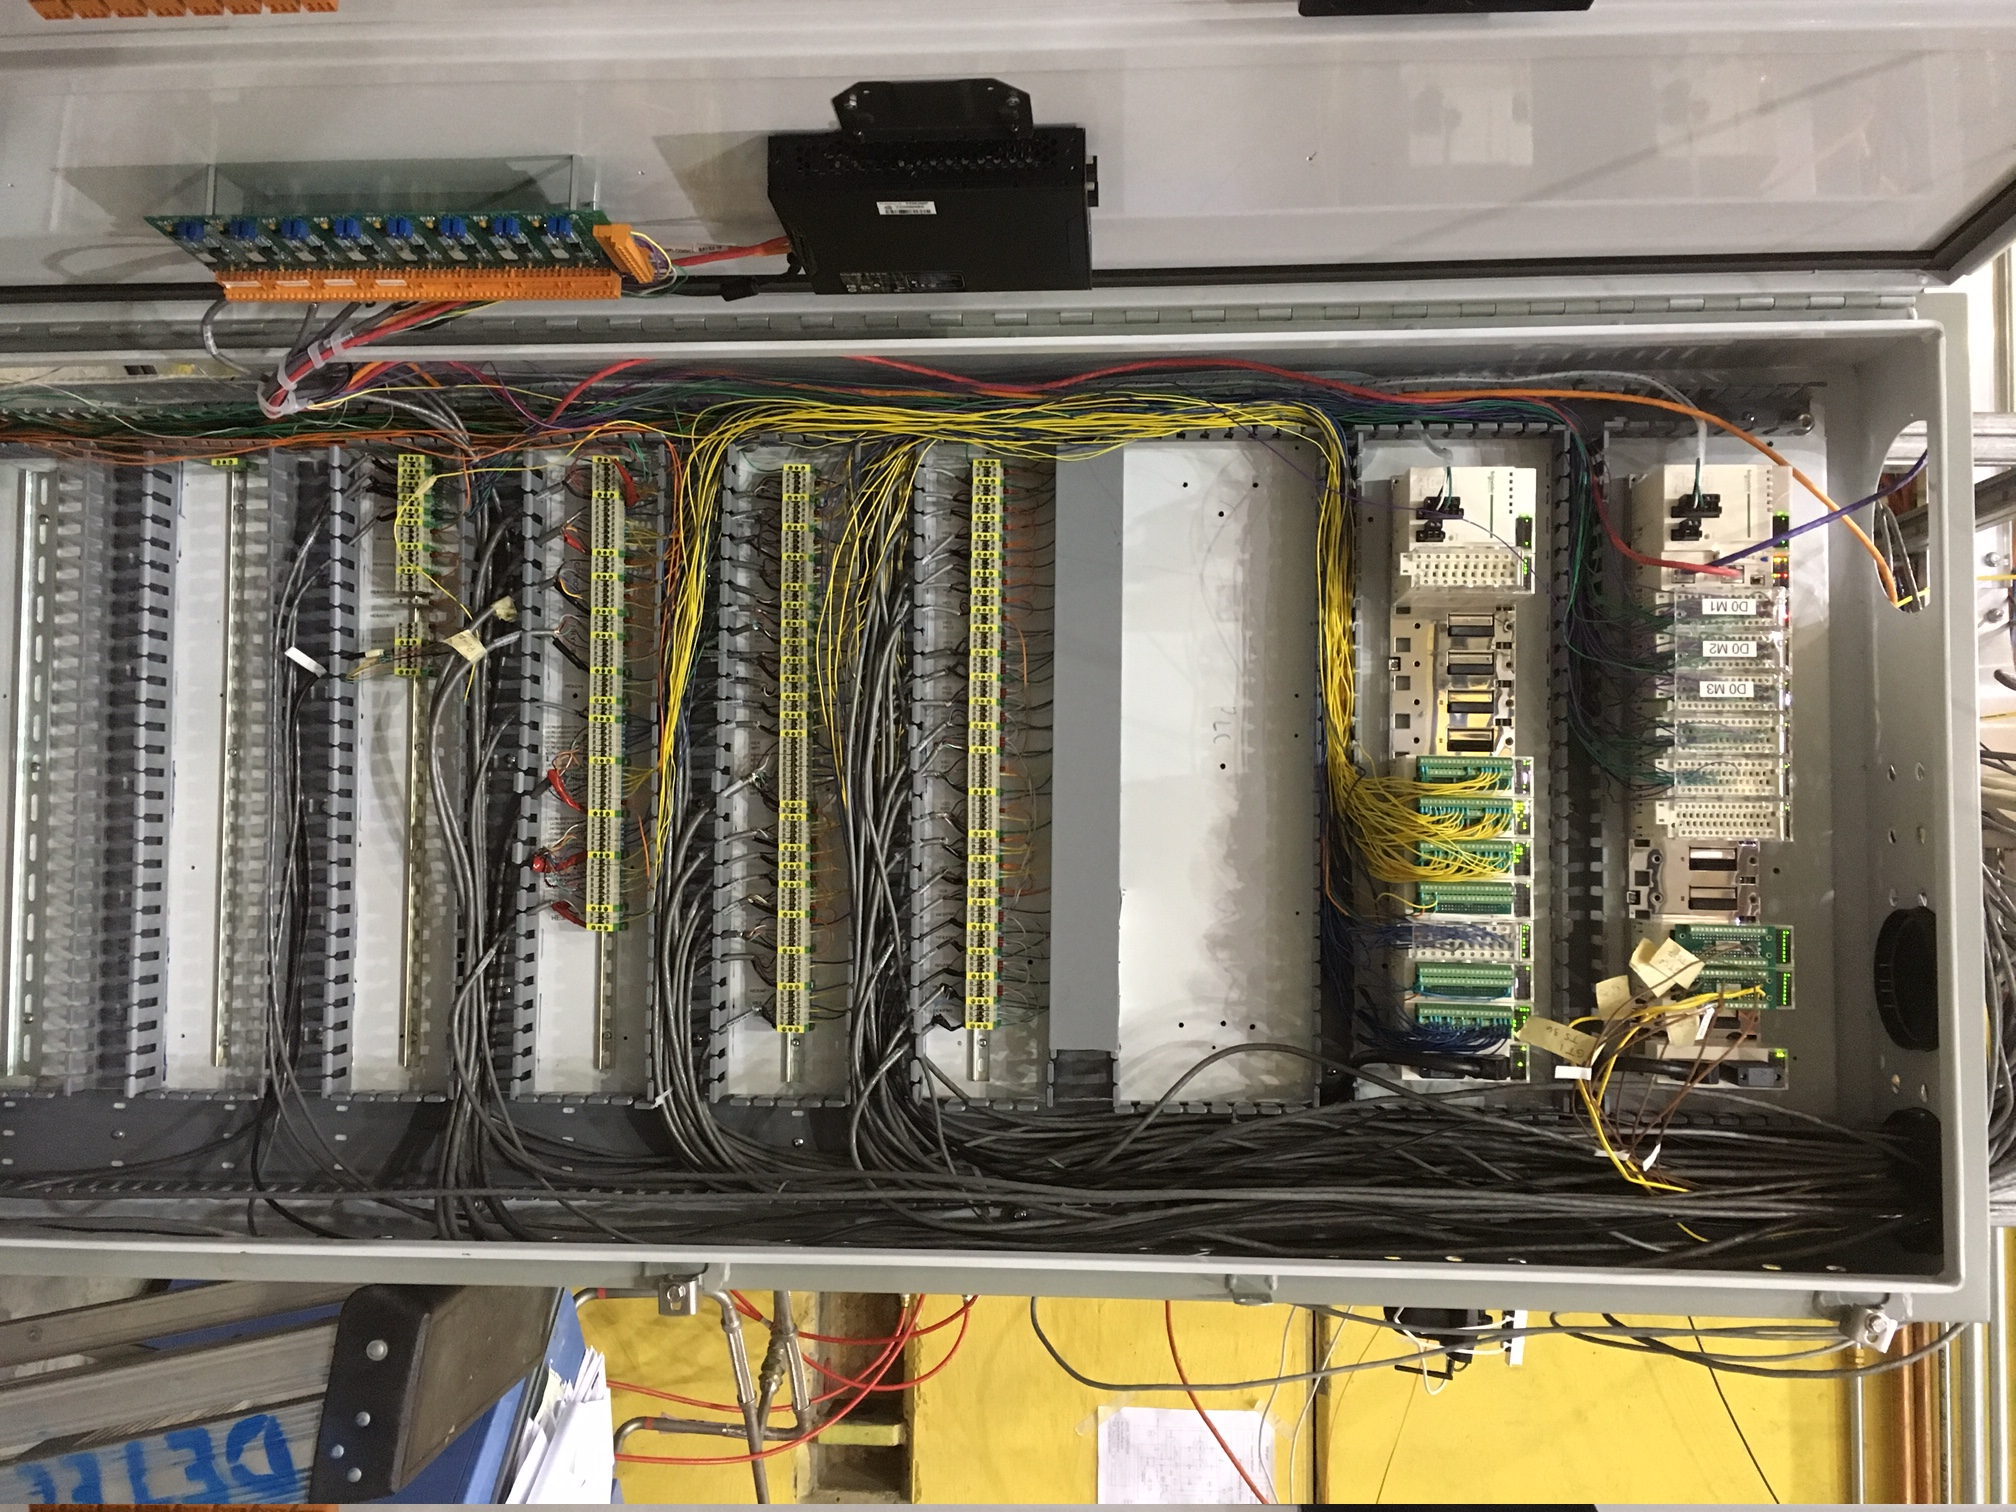
\includegraphics[width=0.8\textwidth, angle = 90]{PLC.JPG}
  \caption{A photograph of the PLC in the meson hall. The grey blocks
    are used to connec the signal from the devices to the computing
    moduels. The first two rows are where the modules are
    located. Each sensor is connected to a specific terminal on a
    specific module. The bottom row is where the power supplies and the
    fuses are positioned. {\bf{insert a new photo}} }
  \label{fig:PLC}
\end{figure}
The communication between the PLC and the screen is handled by EPICS.
The EPICS screen defines the user interface for the controls. It
provides readouts of variables, indications of device status, and
various user input controls for turning devices on/off, resetting
devices, etc. The screen shows the approximate physical layout of the
apparatus being controlled, with each device and its controls placed
in its actual location. The colours of the devices are used to
indicate their current status~\cite{Sean_manual}. Fig.~\ref{fig:epics}
shows the thermal EPICS screen for the TUCAN vertical UCN source
during the November 2017 experimental run. The gas flow screen~(not
shown, very similar to the thermal screen) is intended to contain all
the information about pressures, flows, levels, and controls for pumps and
valves.

\begin{figure}[h!]
  \centering
  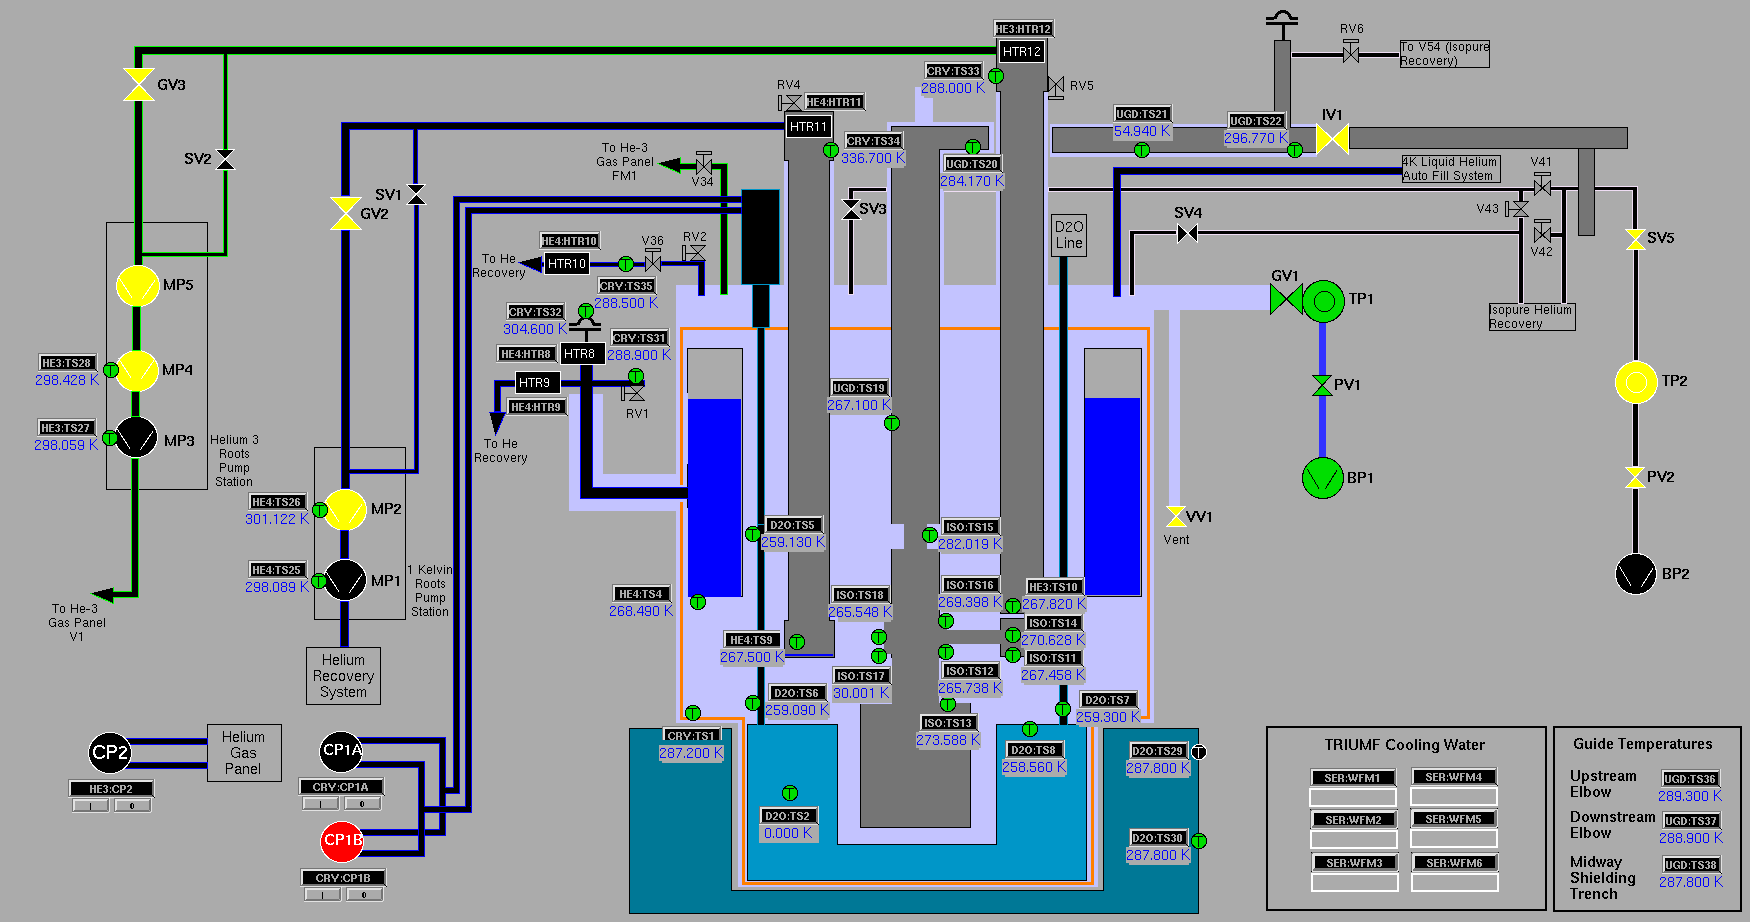
\includegraphics[width=1.0\textwidth]{epics.png}
  \caption{EPICS thermal screen. The approximate location of each
    temperature sensor is shown.The thermal screen is intended to
    contain all information about temperatures, and controls for
    compressors and heaters. }
  \label{fig:epics}
\end{figure}

MIDAS is a modern data acquisition system developed at PSI and TRIUMF
written in C/C++ which runs on all operating systems. MIDAS logs data
in two different ways: History logging where some data is saved
periodically~(every 1-10~s) and can be plotted from history page and
file logging where all data is saved to MIDAS file to be analyzed
later. The TUCAN MIDAS DAQ has a web interface shown in
Fig.~\ref{fig:midas}. The green color indicates that the equipment
frontend is running. Each run can be started by pressing the button at
the top section.

\begin{figure}[h!]
  \centering
  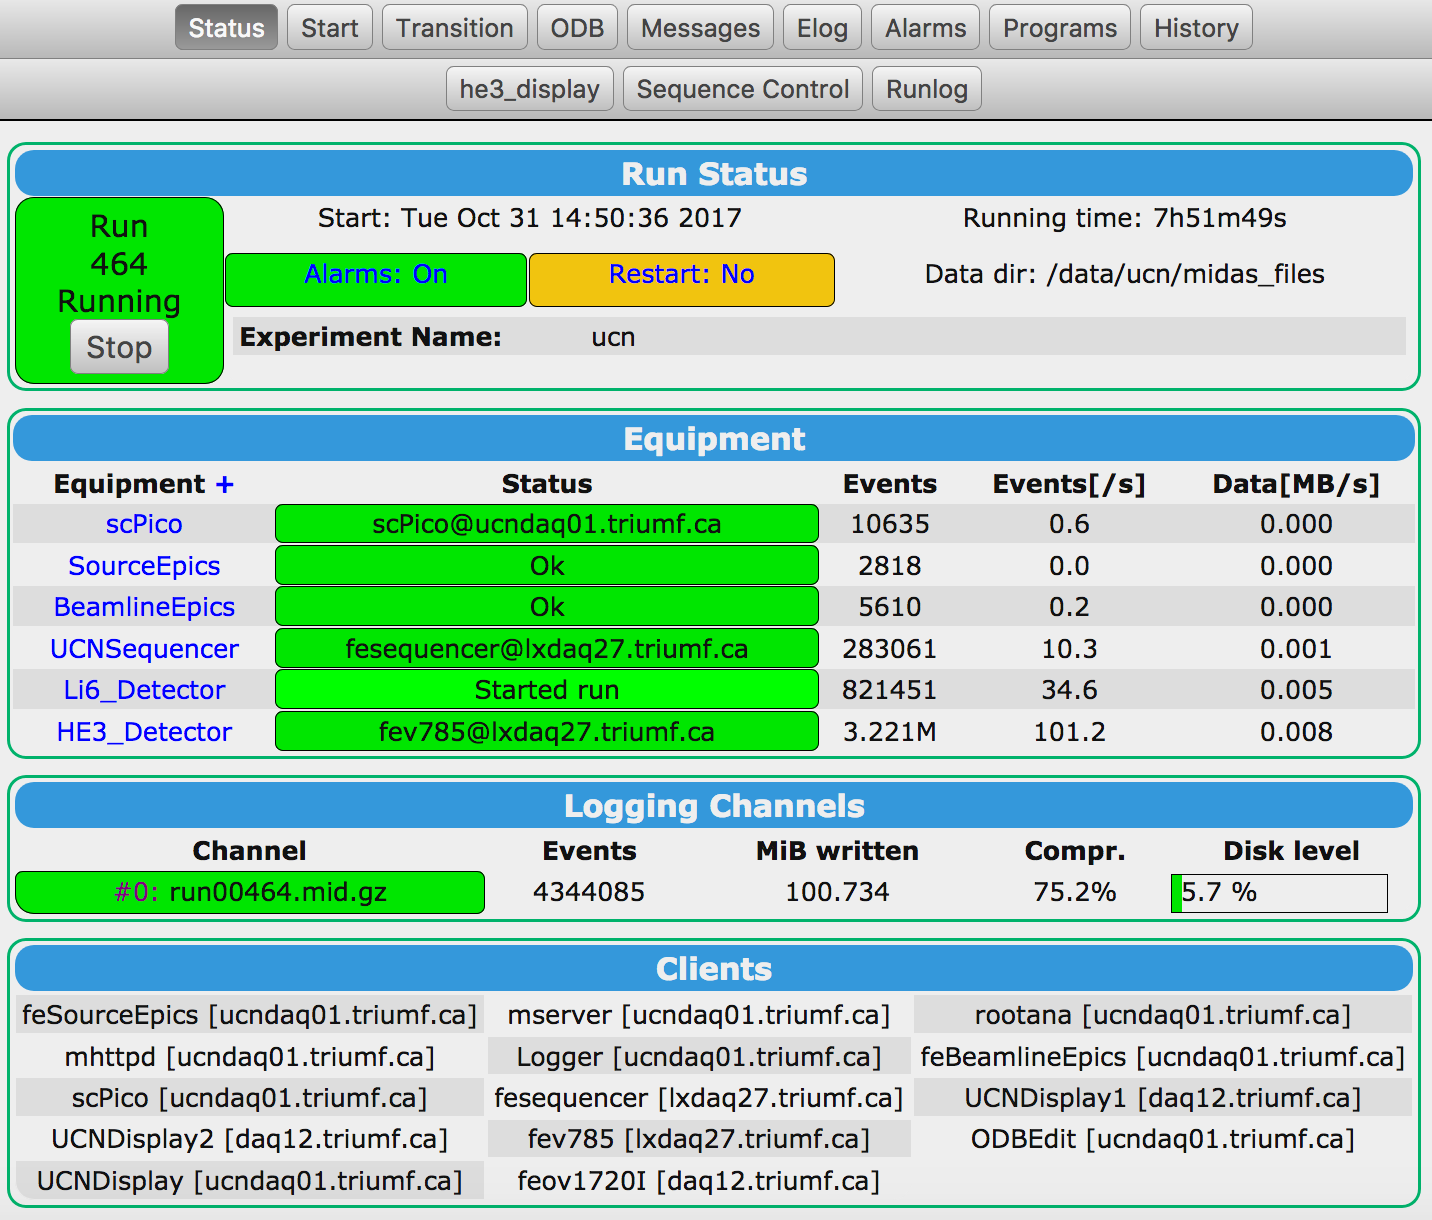
\includegraphics[width=0.8\textwidth]{midas.png}
  \caption{TUCAN MIDAS web interface }
  \label{fig:midas}
\end{figure}

For the 2017 experimental run, each expriment had a unique MIDAS
number. The MIDAS files were then converted to ROOT files for data
analysis. The result of the analysis is presented in
Chapter~\ref{chap:UCNresult}.

\section{UCN Detectors\label{sec:detectors}}
For the TUCAN experimental runs in 2017, a $^6$Li and a $^3$He
detector were used. The main reason for this was to check the
consistency of the result and the performance of each detector. The
brief description of each detector is available below.

\subsection{$^6$Li Detector\label{sec:Li6detector}}
The main detector used during the UCN measurements~(See
Chapter~\ref{chap:UCNresult}) is a $^6\mathrm{Li}$ glass based scintillator
detector designed and built at the University of Winnipeg for the
TUCAN nEDM experiment at
TRIUMF~\cite{jamieson2017characterization}. Since $^6\mathrm{Li}$ has a high
neutron capture cross-section~(order of $10^5$ bn) at UCN energies,
the scintillator glass is doped with it. The charged particles in the
reaction
\begin{equation}
^6Li + n \rightarrow \alpha (2.05~\mathrm{MeV}) + t (2.73~\mathrm{MeV})
\end{equation}
are detected. To reduce the effect of $\alpha$ or triton escaping the
glass, a layer of 60~$\mu$m thick depleted $^6\mathrm{Li}$ glass (GS30), on top
of a layer of 120~$\mu$m thick dopped $^6\mathrm{Li}$ (GS20) were optically
bonded. This design allows the resultant particles to deposit all of
their energy within the scintillating
glass. Table~\ref{tab:scintillator} shows the content and density of
those $^6\mathrm{Li}$ scintillators.

\begin{table}[h!]
  \centering
  \label{tab:scintillator}
  \begin{tabular}{|c|c|c|}
    \hline
    Scintillator & GS20~($^6\mathrm{Li}$ Enriched) & GS30~( $^6\mathrm{Li}$ depleted) \\
    \hline
    Total Li content (\%) & 6.6 & 6.6 \\
    \hline
    $^6\mathrm{Li}$ fraction (\%) & 95 & 0.01 \\
    \hline
    $^6\mathrm{Li}$ desity~(cm$^{-3}$) & $1.716 \times 10^{22}$ & $1.806 \times 10^{18}$ \\
    \hline
  \end{tabular}
  \caption{Properties of the glass scintillators}
\end{table}


Making the scintillating Li glass as thin as possible reduces the
sensitivity to $\gamma$-ray scintillating backgrounds and and thermal
neutron captures. The mean range of the $\alpha$ is 5.3~$\mu$m and the
mean range of the triton is 34.7~$\mu$m. This means that if the
thickness of the scintillator is less than 50~$\mu$m, the resultant
particles escape before stopping which gives rise to an efficiency
loss.  In order to handle high UCN rates of up to \~1~MHz, the
$^6\mathrm{Li}$ detector face is segmented into 9 tiles~(See
Fig.~\ref{fig:Li6detector}). The scintillation light is then guided
through ultra-violet transmitting acrylic light-guide to its
corresponding Photomultiplier Tube~(PMT) outside the vaccum region of
the detector.

\begin{figure}[h]
  \centering
  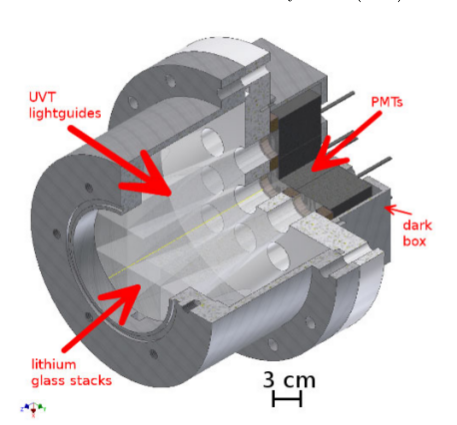
\includegraphics[width=0.5\textwidth]{Li6detector.png}
  \caption{3D drawing of the $^6$Li detector and its enclosure. The
    enclosure is made of Al, and the rim of the adapter flange which
    UCN can hit is ccoated with 1~$\mu$m Ni by thermal evaporation. }
  \label{fig:Li6detector}
\end{figure}

The data acquisition with this detector includes a CAEN V1720
digitizer which has a Pulse-Shape Discrimination~(PSD) firmware that
triggers on pulses below a certain threshold for each channel. Every
4~ns the digitizer samples the waveform which is then digitized to a
voltage on a 2~V scale into an ADC value between 0 and 4096. Each
channel of the digitizer sends a trigger whenever the number of counts
in the ADC goes below a certain baseline~(pedestal) value. The PSD
calculates the sum of the signal below the baseline for two time
windows: $t_s = 40$~ns (short gate) and $t_L = 200$~ns~(long
gate). The short gate is chosen in a way to contain all of the charge
for the $\gamma$-ray interactions in the light-guide. The ADC sum for
during the long gate below the baseline is calle $Q_L$~(read charge
long) and for during the short gate below the baseline is called
$Q_S$. Charge long has the total charge deposti for the neutron
capture events. The PSD value is defined as
\begin{equation}
  \label{eq:psd}
  \mathrm{PSD} = \frac{\left( Q_L - Q_S\right)}{Q_L}
\end{equation}  
which is the amount of charge in the tail of an event.

Jamieson {\it{et al.}} showed that the absolute efficiency of this
detector is $89.7^{+1.3}_{-1.9}$~\% with a background contamination of
$0.3 \pm 0.1$~\%~\cite{jamieson2017characterization}. The detector is
stable at the 0.06~\% level or better, and that the variation in the
efficiency between the detector tiles is less than 5~\%.
\subsection{$^3$He Detector}

The $^3$He detector used for the data acquisition is a Dunia-10 type
which was shipped from RCNP.  $^3$He provides an effective neutron
detector material for neutron detection by absorbing neutrons via the
following reaction

\begin{equation}
  \label{eqn:he3}
n + ^3\mathrm{He} \rightarrow p + t + 674~\mathrm{keV}.
\end{equation}

Before the start of the experiment, the $^3$He detector was tested
with an AmBe source and it showed consistent result with what was
observed at RCNP. The detector was surrounded with parafin blocks to
moderate the neutrons~(see Fig.~\ref{fig:he3detector}.

\begin{figure}[h]
  \centering
  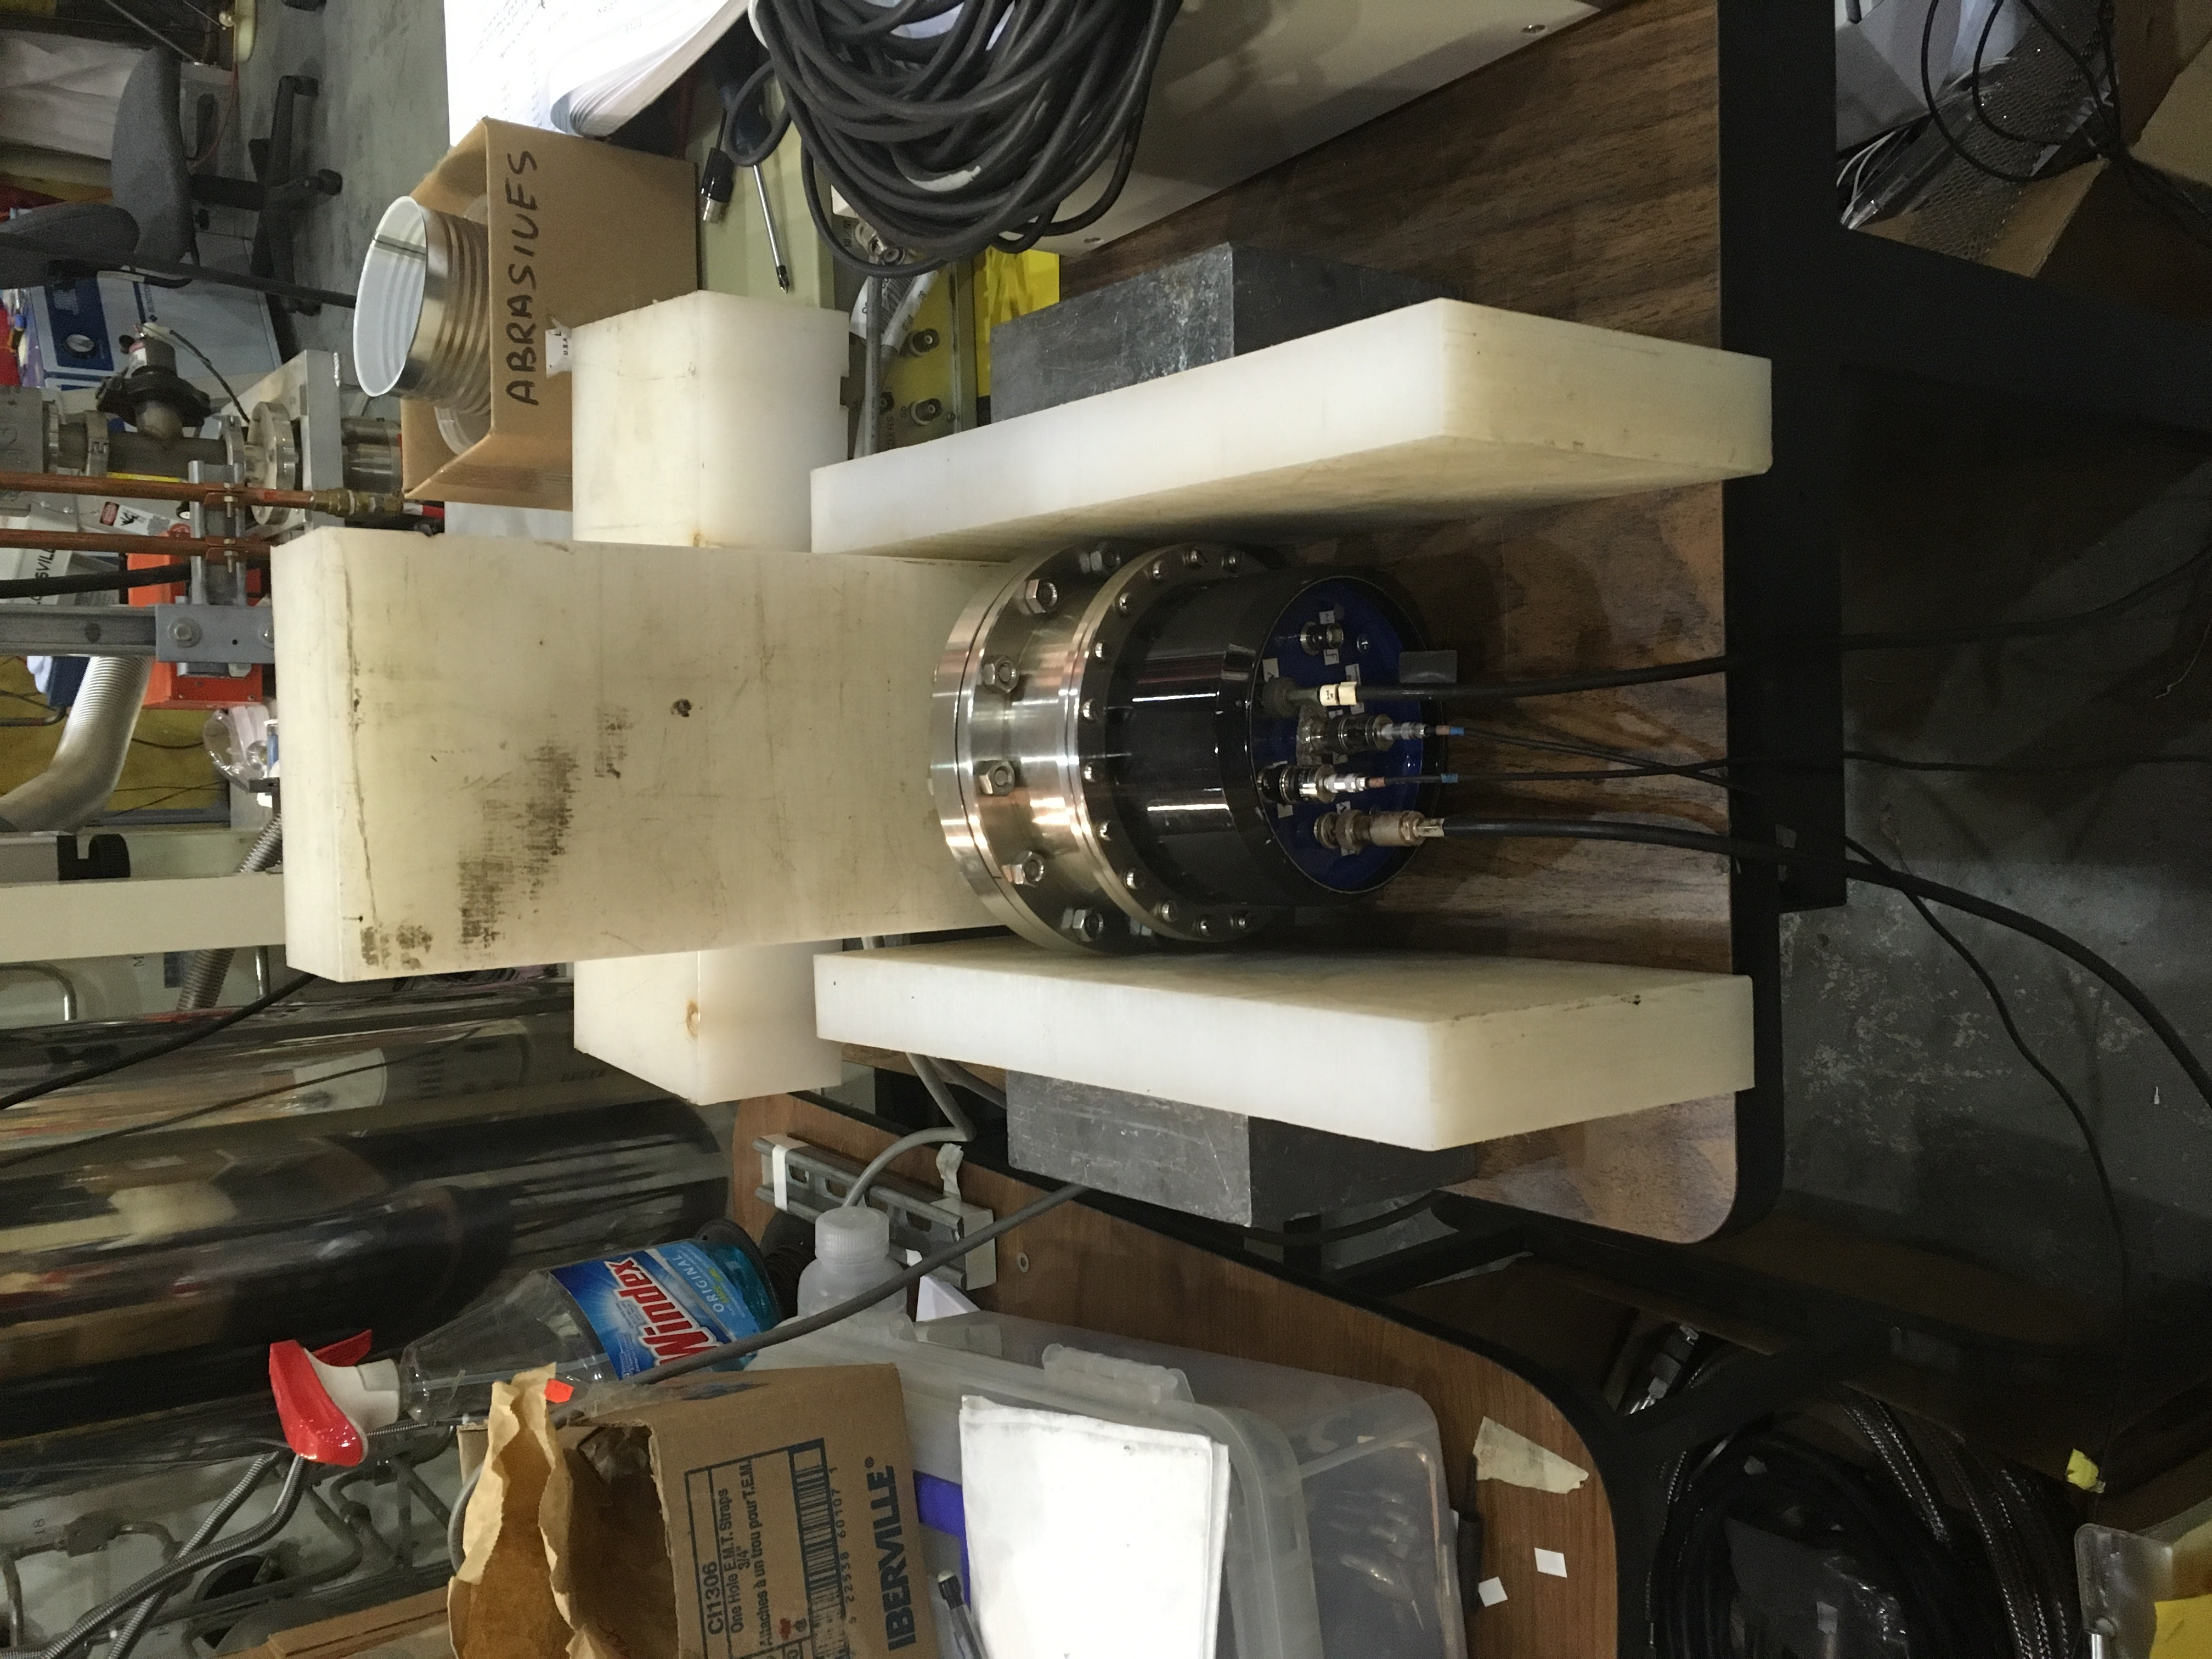
\includegraphics[width=0.5\textwidth, angle = 270]{he3detector.png}
  \caption{$^3$He detector and parafin blocks for neutron
    moderation.}
  \label{fig:Li6detector}
\end{figure}

More detail about the $^3$He detector could be found in
Ref.~\cite{matsumiya_thesis}. The result of the comparison between the
$^3$He and $^6$Li detectors are available in
Sec.~\ref{sec:detector_comparison}.

%\begin{description}
%\item{An intro to whatever goes into this chapter}

%\item{Start by showing a nice drawing and then talk about each
 % componet of the facility:}
  
%\item{about proton beam that we get, the magnets and basically how the
%  beam reaches the target and how it looks like (Where can I get this
%  information? Is it written somewhere?)}
  
%\item{A short introduction to say the stages of UCN production and why
%  we need the vertical cryostat (Link to the next stage)}
  
%\item{It also has to be mention that it is the same vertical sourcse
%  as was used at the RCNP and some modifications were made to meet the
%  requirements at triumf. (Where can I find what modifications were
%  made?) Agian this has to be just as a link to the next chapter(maybe?)}
  
%\item{The target and shielding (with pictures?), only a few
%  paragraphs}
  
%\item{Moderation: D2O system (I can use Ryohei's thesis I guess)}
  
%\item{conversion. There is a whole chapter dedicated to the UCN
%  cryogenics. I have to go through details (not too much) of how the
%  cryostat works. I can borrow some infromation from Ryohei's
%  thesis. I am not sure how much of it is related to the next
%  chapter.}
 

%\item{Data acquisition system, epics and plc, I guess there are useful
%  informaion in Sean Vanbergen's report that I can use for this
%  section}
  
%\item{what else?}

%\end{description}
